\documentclass[border=5pt]{standalone}
\usepackage{tikz}
\usepackage{amsmath}
\begin{document}
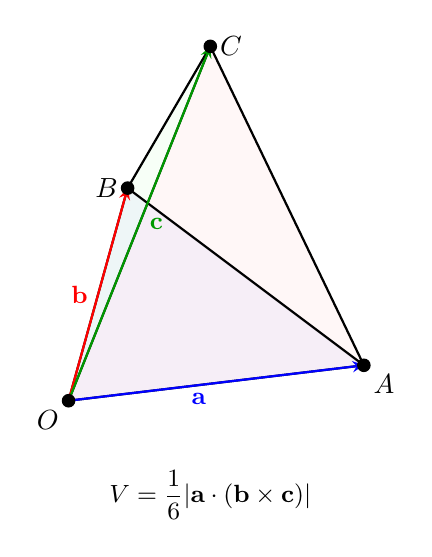
\begin{tikzpicture}[scale=1.5, >=stealth]
  % 3D tetrahedron

  % Vertices
  \coordinate (O) at (0,0);
  \coordinate (A) at (2.5,0.3);
  \coordinate (B) at (0.5,1.8);
  \coordinate (C) at (1.2,3.0);

  % Fill faces
  \fill[blue!10, opacity=0.5] (O) -- (A) -- (B) -- cycle;
  \fill[red!10, opacity=0.3] (O) -- (A) -- (C) -- cycle;
  \fill[green!10, opacity=0.3] (O) -- (B) -- (C) -- cycle;

  % Edges
  \draw[thick] (O) -- (A);
  \draw[thick] (O) -- (B);
  \draw[thick] (O) -- (C);
  \draw[thick] (A) -- (B);
  \draw[thick] (A) -- (C);
  \draw[thick] (B) -- (C);

  % Vectors from origin
  \draw[->, thick, blue] (O) -- (A) node[midway, below left, font=\small] {$\mathbf{a}$};
  \draw[->, thick, red] (O) -- (B) node[midway, left, font=\small] {$\mathbf{b}$};
  \draw[->, thick, green!60!black] (O) -- (C) node[midway, right, font=\small] {$\mathbf{c}$};

  % Vertices
  \filldraw[black] (O) circle (1.5pt) node[below left] {$O$};
  \filldraw[black] (A) circle (1.5pt) node[below right] {$A$};
  \filldraw[black] (B) circle (1.5pt) node[left] {$B$};
  \filldraw[black] (C) circle (1.5pt) node[right] {$C$};

  % Volume formula
  \node[font=\small] at (1.2, -0.8) {$V = \dfrac{1}{6}|\mathbf{a}\cdot(\mathbf{b}\times\mathbf{c})|$};
\end{tikzpicture}
\end{document}
